\documentclass[10pt]{beamer}

\input{/Users/daniel/Documents/LaTeX/beamer-style.tex}


\title{SGBD - 2\textsuperscript{e}}
\subtitle{Chapitre 2 : Modèle relationnel}
\date{\today}
\author{Daniel Schreurs}
\institute{Haute École de Province de Liège}
%\titlegraphic{\hfill\includegraphics[height=1.5cm]{logo.eps}}

\begin{document}

\maketitle

\setbeamerfont{subsection in toc}{size=\small}
\setbeamerfont{subsubsection in toc}{size=\normalsize}
\setbeamertemplate{section in toc}[sections numbered]
\setbeamertemplate{subsection in toc}[subsections numbered]
\setbeamertemplate{subsubsection in toc}[subsubsections numbered]
\begin{frame}[allowframebreaks]{Table des matières du chapitre}
    \tableofcontents[subsectionstyle=show/show/hide,subsubsectionstyle=show/show/hide,]
\end{frame}

\section{Introduction}
\tocss

\subsection{Différents modèles}
\begin{frame}{\secname : \subsecname}
    \begin{itemize}
        \item Modèle réseau
        \item Modèle hiérarchique
        \item \textbf{Modèle relationnel}
        \item Modèle Objet - rel
    \end{itemize}
    \metroset{block=fill}
    \begin{alertblock}{Important}
        Nous n'étudierons, dans le cadre de ce cours, que le modèle relationnel.
    \end{alertblock}
\end{frame}

\subsection{Le modèle relationnel}
\begin{frame}{\secname : \subsecname}
    En 1970, un mathématicien, \href{https://fr.wikipedia.org/wiki/Edgar_Frank_Codd}{E.F. Codd}, publie un article qui établit les bases du modèle relationnel.
    Ce modèle constitue un des apports les plus remarquables à la gestion de l’information que l’on peut résumer en 4 points :
    \begin{itemize}
        \item Rigueur des concepts de base
        \item Simplicité des concepts de base
        \item Puissance des opérateurs de manipulation
        \item Diminution des coûts de développement et de maintenance
    \end{itemize}
\end{frame}

\subsubsection{Rigueur des concepts de base}
\begin{frame}{\subsecname : \subsubsecname}
    Le modèle relationnel s’appuie sur une base formelle : la théorie des ensembles ou la théorie des prédicats.
    \begin{itemize}
        \item Un \textbf{ensemble} est une collection, un regroupement d’objets, de nombres, d’identités concrètes ou abstraites;
        \item Les objets particuliers qui appartiennent à un ensemble sont appelés les \textbf{éléments} de cet ensemble;
        \item On peut représenter graphiquement les ensembles et les opérations sur les ensembles par des \textbf{diagrammes de Venn}.
    \end{itemize}
\end{frame}

\begin{frame}{\subsecname : \subsubsecname}
    \metroset{block=fill}
    \begin{alertblock}{Important}
        Le modèle relationnel s’appuie sur une base formelle : la théorie des ensembles ou la théorie des prédicats\footnote{Un prédicat est une phrase qui peut comporter des paramètres et qui peut être vraie ou fausse}.
    \end{alertblock}
    \begin{itemize}
        \item Des prédicats : $P, Q$
        \item Des connecteurs logiques : $\land, \lor$
        \item Des opérateurs  : $+,-,\setminus$, etc..
        \item Des quantificateurs : $\exists, \forall$
        \item Des variables : $x,y$
        \item Des constantes : $a,b$
        \item Des fonctions : $f,g$
    \end{itemize}
\end{frame}

\begin{frame}{\subsecname : \subsubsecname}
    Un petit exemple :
    $$\forall x, \exists y | amis(x,y) \land amis(x,mere(y))$$
\end{frame}

\subsubsection{Simplicité des concepts de base}
\begin{frame}{\subsecname : \subsubsecname}
    Une relation est un ensemble, au sens mathématique, qui va être visualisé sous la forme d’une table.
    Il en résulte :
    \begin{itemize}
        \item Facilité d’apprentissage (par développeurs et utilisateurs)
        \item Plus grande communicabilité entre informaticiens et non-informaticiens
        \item Plus aucune référence à une méthode d’accès à un fichier ou organisation particulière des données sur les supports.
    \end{itemize}
\end{frame}

\subsubsection{Puissance des opérateurs de manipulation}
\begin{frame}{\subsecname : \subsubsecname}
    \textbf{Les opérateurs relationnels sont des opérateurs ensemblistes.}
    L’application d’un opérateur à une ou plusieurs relations donne toujours une relation qui peut, à son tour, servir d’argument à un autre opérateur
    \metroset{block=fill}
    \begin{alertblock}{Important}
        \begin{itemize}
            \item notion de fermeture
            \item Non procédural : on dit ce que l'on veut obtenir, mais pas comment
        \end{itemize}
    \end{alertblock}
\end{frame}
\subsubsection{Diminution des coûts de développement et de maintenance}
\begin{frame}{\subsecname : \subsubsecname}
    Il a été estimé que le gain temps de développement d’une application de gestion varie entre 25 et 75\% avec l’utilisation d’un SGBD relationnel.
\end{frame}

\subsubsection{Codd}
\begin{frame}{\subsecname : \subsubsecname}
    Le modèle relationnel de Codd repose sur 3 piliers :
    \begin{itemize}
        \item Les \textbf{objets}  : les éléments de base;
        \item Les \textbf{règles d’intégrité} : permettent de faire respecter le modèle des données;
        \item Les \textbf{opérateurs} : offrent la possibilité de manipuler la base de données;
    \end{itemize}
\end{frame}

\subsubsection{Les objets}
\begin{frame}{\subsecname : \subsubsecname}
    \begin{itemize}
        \item Relation Domaine/attribut
        \item Clé primaire
        \item Domaine primaire  (clé étrangère)
    \end{itemize}
\end{frame}
\subsubsection{Les contraintes}
\begin{frame}{\subsecname : \subsubsecname}
    \begin{itemize}
        \item Contraintes d'intégrité de domaine
        \item Intégrité d’entité ou de relation
        \item Intégrité de référence
    \end{itemize}
\end{frame}
\subsubsection{Opérateurs}
\begin{frame}{\subsecname : \subsubsecname}
    \begin{itemize}
        \item Opérateurs sémantiques (liés aux domaines)
        \item Opérateurs ensemblistes : union, différence, produit cartésien
        \item Opérateurs relationnels : restriction (sélection), projection,
        \item Opérateurs additionnels : jointure, intersection, division
    \end{itemize}
\end{frame}


\subsection{Base de données}
\subsubsection{Ouvrages}
\begin{frame}{\subsecname : \subsubsecname}
    \begin{figure}
        \begin{center}
            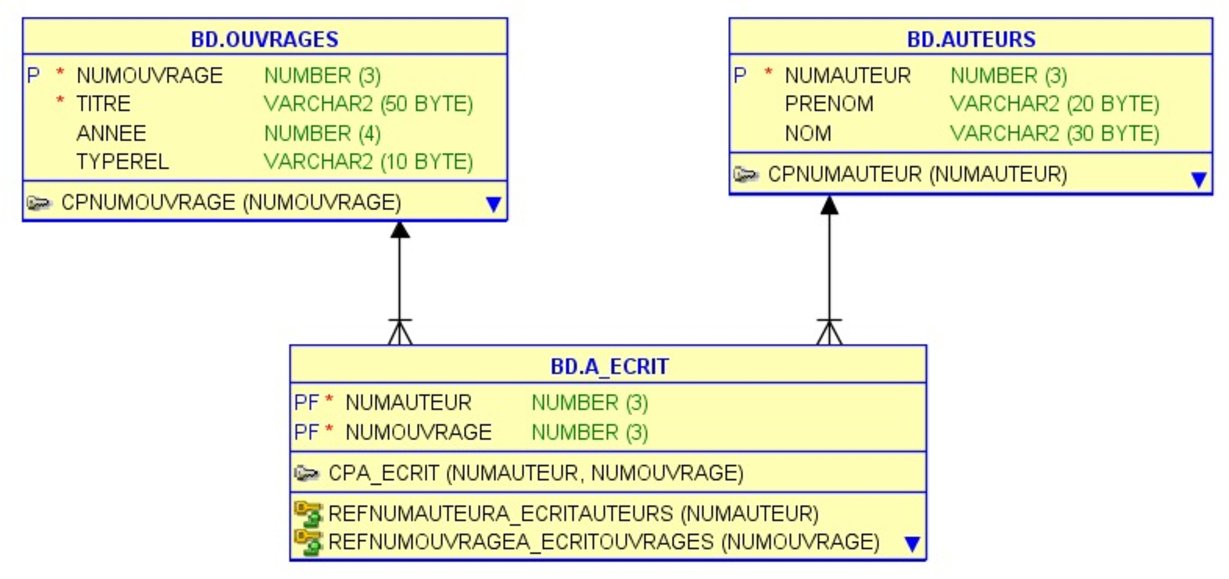
\includegraphics[width=0.8\textwidth]{../assets/img/bd_ouvrages.pdf}
            \caption*{Base de données "Bandes Dessinées" utilisée dans les exemples}
            \label{Fig:bd_ouvrages}
        \end{center}
    \end{figure}
\end{frame}

\begin{frame}{\subsecname : \subsubsecname}
    \begin{figure}
        \begin{center}
            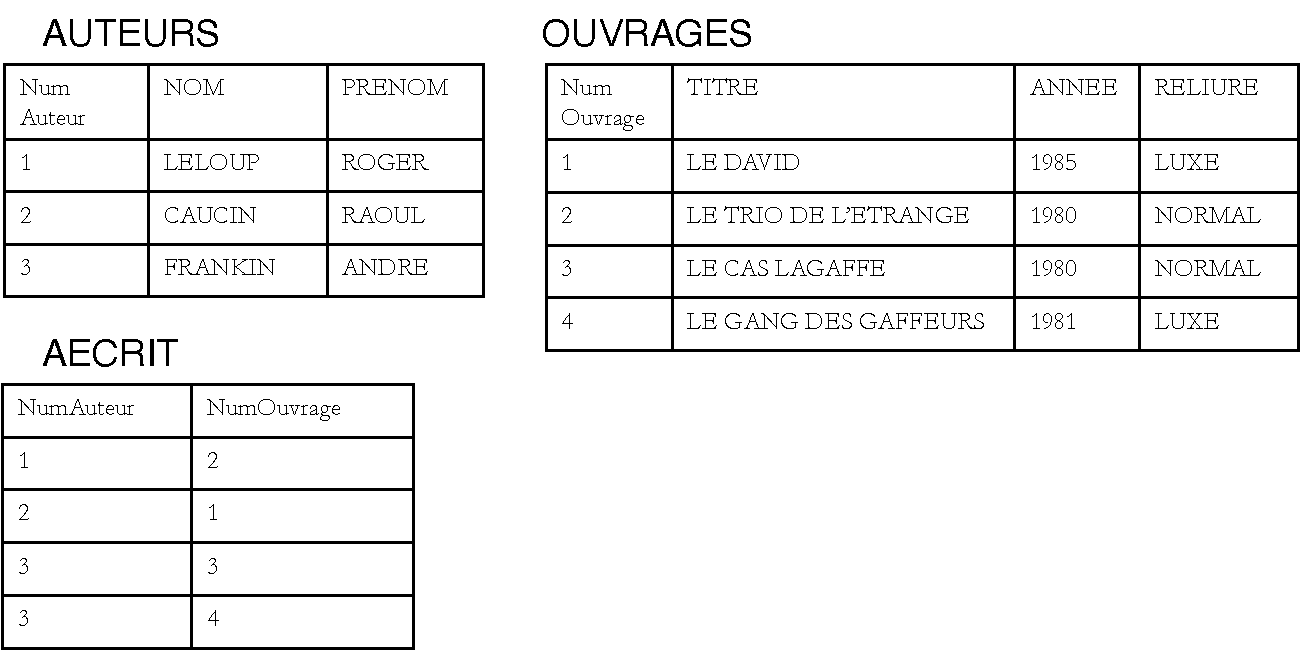
\includegraphics[width=0.8\textwidth]{../assets/img/bd_ouvrages--data.pdf}
            \caption*{Base de données "Bandes Dessinées" utilisée dans les exemples}
            \label{Fig:bd_ouvrages--data}
        \end{center}
    \end{figure}
\end{frame}
\section{Relation, domaine et attribut}
\tocss
\subsection{Relation}

\begin{frame}{\secname : \subsecname}
    \begin{itemize}
        \item La relation $AUTEURS$ est représentée sous forme d’une table.
        \item Une ligne de la table constitue un élément de la relation.
        \item La relation ou table possède 3 colonnes ou attributs
        \item Chaque attribut a une valeur qui fait partie d’un ensemble de valeurs permises (domaine de l’attribut).
        \item Exemples :
              \begin{itemize}
                  \item NumAuteur : domaine = l’ensemble des entiers positifs (D1)
                  \item Nom : domaine = l’ensemble des chaînes de caractères de longueur 30 (D2)
              \end{itemize}
        \item Une ligne quelconque de la table $AUTEURS$ est constituée de $(V1, V2, V3)$ | $V1 \in D1 \land V2 \in D2 \land V3 \in D3$
        \item La table $AUTEURS$ est un sous-ensemble de toutes les combinaisons possibles, donc un sous-ensemble du produit cartésien $D1 * D2 * D3$
    \end{itemize}
\end{frame}

\begin{frame}{\secname : \subsecname}
    \metroset{block=fill}
    \begin{alertblock}{Important}
        Une RELATION $R$ est un sous-ensemble du produit cartésien de $n$ ensembles $D_i$ appelés DOMAINES.
    \end{alertblock}
    Une relation est donc un ensemble d’éléments de la forme
    $$
        (v_1,v_2,v_3,..., v_n) | 1\leq i \leq n, v_i \in D_i
    $$
    que l’on appelle n-uplet ou tuple ou encore ligne. $n$ est appelé le degré de la relation.
\end{frame}

\begin{frame}{\secname : \subsecname}
    Une relation étant un ensemble, elle peut être définie de manière :
    \begin{itemize}
        \item Extensive : en donnant la liste de tous les tuples la composant : $AEcrit = \{(1, 2), (2, 1), (3, 3), (3, 4)\}$
        \item Intensive : en donnant le prédicat d’appartenance d’un tuple à R : $AEcrit = \{ (x, y) | ... \}$

    \end{itemize}
\end{frame}
\subsection{Domaine}

\begin{frame}{\secname : \subsecname}

    \metroset{block=fill}
    \begin{alertblock}{Important}
        Un domaine représente l’ensemble des valeurs admissibles pour une composante d’une relation.
    \end{alertblock}
    Syntaxe $\neq$ Sémantique
\end{frame}

\begin{frame}{\secname : \subsecname}
    Les relations sont définies à partir de domaines.
    Pour définir une base de données relationnelle, on commence par définir les domaines.
    \begin{itemize}
        \item Domaine NumeroAuteur = entier compris entre 1 et 100
        \item Domaine NomAuteur = chaîne de caractères
        \item Domaine PrenomAuteur = chaîne de caractères
        \item Domaine NumeroOuvrage = entier compris entre 1 et 500
        \item Domaine TitreOuvrage = chaîne de caractères
        \item Domaine AnneeEdition = entier $\geq$ 1900
        \item Domaine TypeReliure = $\{'NORMAL', 'LUXE', 'CARTONNE', 'BROCHE'\}$
    \end{itemize}
\end{frame}

\begin{frame}{\secname : \subsecname}
    Définition des  relations sur base des domaines :
    Relation AUTEURS composée des attributs :
    \begin{itemize}
        \item NumAuteur : défini sur NumeroAuteur,
        \item Nom : défini sur NomAuteur,
        \item Prenom : défini sur PrenomAuteur;
    \end{itemize}
    Relation OUVRAGES composée des attributs :
    \begin{itemize}
        \item NumOuvrage : défini sur NumeroOuvrage,
        \item Titre : défini sur TitreOuvrage,
        \item Année : défini sur AnneeEdition,
        \item Reliure : défini sur TypeReliure
    \end{itemize}
    ...
\end{frame}

\begin{frame}{\secname : \subsecname}
    Deux domaines sont déclarés compatibles s’ils sont sémantiquement comparables, c’est-à-dire si les ensembles qui les définissent ne sont pas disjoints.
\end{frame}

\begin{frame}{\secname : \subsecname}
    \begin{itemize}
        \item En particulier, deux domaines identiques ou liés par inclusion sont compatibles.
              Exemple : les domaines VilleEurope et VilleBelge, tous deux de type chaîne de caractères sont liés par inclusion et donc compatibles\footnote{Puisque toutes les villes de la Belgique sont aussi de villes de l'Europe.}.
        \item Exemple de domaines non compatibles : NumeroAuteur et NumeroOuvrage sont incompatibles même s’ils sont définis au moyen de types de données comparables (des nb entiers)
    \end{itemize}
\end{frame}

\begin{frame}{\secname : \subsecname}
    \begin{itemize}
        \item Les noms des domaines et des attributs correspondants ne sont pas les mêmes.
        \item Il est possible d’avoir dans une même table deux attributs différents issus du même domaine
        \item Par contre, les attributs d’une relation doivent tous être différents.
    \end{itemize}
\end{frame}

\section{Clé primaire}
\tocss
\subsection{Objectifs}
\begin{frame}{\secname : \subsecname}
    \begin{itemize}
        \item Une relation est un ensemble. Il doit être possible de distinguer tous les éléments (tuples) de la relation.
        \item Un attribut ou un groupe d’attributs va jouer le rôle d’identifiant de la relation : c’est la \textbf{clé primaire}.
        \item Une valeur de clé primaire permet d’identifier de manière unique un tuple d’une relation.
    \end{itemize}
\end{frame}

\subsection{Définition}
\begin{frame}{\secname : \subsecname}
    \metroset{block=fill}
    \begin{alertblock}{Important}
        Une clé primaire est un ensemble d’attributs, K, vérifiant la double propriété :
        \begin{itemize}
            \item Unicité : les valeurs de clés primaires sont uniques et non nulles\footnote{$NULL$ ne veut pas dire $""$ ou $0$ mais \emph{absence de valeur}.};
            \item Minimalité : aucun attribut composant K ne peut être enlevé sans perdre la propriété d’unicité.
        \end{itemize}
    \end{alertblock}
\end{frame}

\subsection{Exercice}
\begin{frame}{\secname : \subsecname}
    Spécifier les clés primaires dans le schéma suivant :
    \begin{figure}
        \begin{center}
            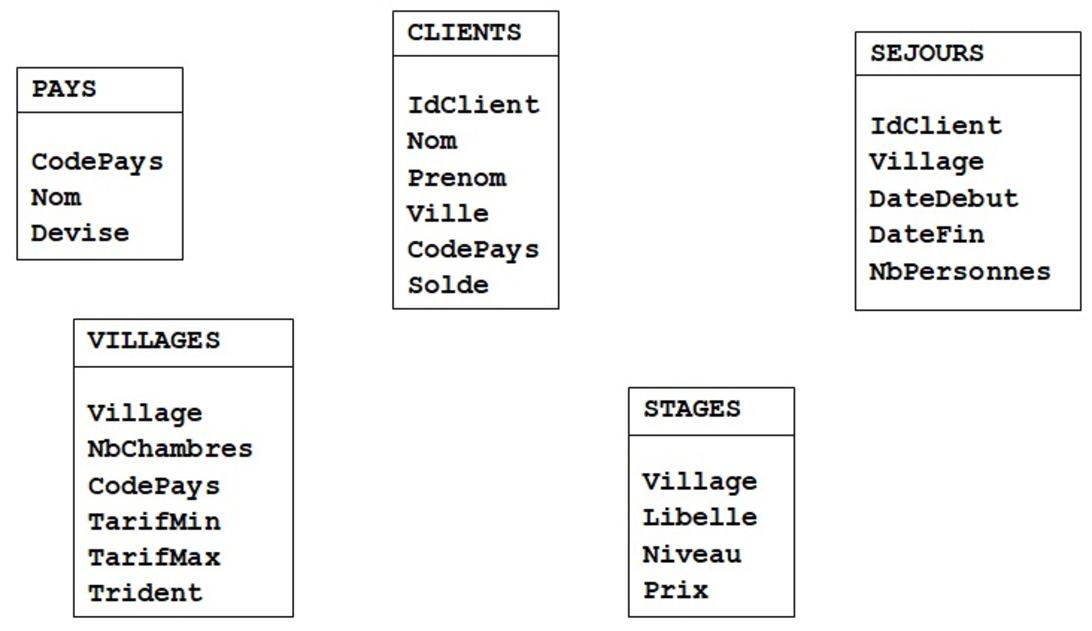
\includegraphics[width=0.75\textwidth]{../assets/img/db_villes.pdf}
            \caption*{Structure d’une DB pour des séjours}
            \label{Fig:db_villes.pdf}
        \end{center}
    \end{figure}
\end{frame}

\section{Domaine primaire - clé étrangère}
\subsection{Définition}
\begin{frame}{\secname : \subsecname}
    \metroset{block=fill}
    \begin{alertblock}{Important}
        Un domaine primaire est un domaine sur lequel une clé primaire est définie.
    \end{alertblock}
    Exemple : NumeroAuteur et NumeroOuvrage sont des domaines primaires.
\end{frame}
\begin{frame}{\secname : \subsecname}
    \metroset{block=fill}
    \begin{alertblock}{Important}
        Un attribut qui n’est pas clé primaire, mais qui est défini sur un domaine primaire est appelé une clé étrangère\footnote{La notion de clé étrangère permet d’exprimer les associations entre entités.}.
    \end{alertblock}
    Exemple : NumAuteur et NumOuvrage, dans la relation AEcrit, sont des clés étrangères.
\end{frame}


\section{Intégrité de domaine}
\subsection{Définition}
\begin{frame}{\secname : \subsecname}
    Il existe deux grandes classes de contraintes d’intégrité :
    \begin{itemize}
        \item Les \textbf{contraintes structurelles} dépendant du modèle de données (intégrité de domaine, d’entité ou de relation et de référence);
        \item Les \textbf{contraintes applicatives} liées à l’univers réel modélisé.
    \end{itemize}
\end{frame}

\begin{frame}{\secname : \subsecname}
    \metroset{block=fill}
    \begin{alertblock}{Important}
        L’intégrité de domaine porte sur le contrôle syntaxique et sémantique des valeurs présentes dans un attribut : seules les valeurs appartenant au domaine de l’attribut sont autorisées\footnote{Ce type de vérification se fait lors du chargement initial de la base de données comme pendant toute manipulation de celle-ci.}.
    \end{alertblock}
\end{frame}

\section{Intégrité d’entité ou de relation}
\subsection{Définition}
\begin{frame}{\secname : \subsecname}
    \metroset{block=fill}
    \begin{alertblock}{Important}
        L’intégrité d’entité ou de relation concerne les valeurs de la clé primaire d’une relation qui doivent être uniques et toujours définies (non nulles).
    \end{alertblock}
\end{frame}

\section{Intégrité de référence}
\subsection{Exercice}
\begin{frame}{\secname : \subsecname}
    Spécifier les clés primaires et les clés étrangères dans le schéma suivant :
    \begin{figure}
        \begin{center}
            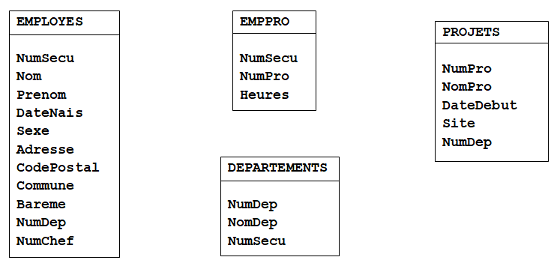
\includegraphics[width=0.75\textwidth]{../assets/img/bd_employe.png}
            \label{Fig:bd_employe}
        \end{center}
    \end{figure}
\end{frame}

\begin{frame}{\secname : \subsecname}
    Spécifier les clés primaires et les clés étrangères dans le schéma suivant :
    \begin{figure}
        \begin{center}
            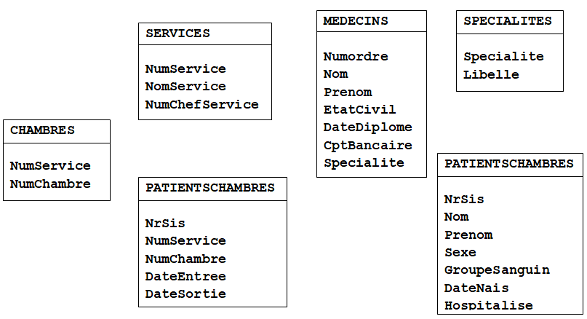
\includegraphics[width=0.75\textwidth]{../assets/img/bd_hopital.png}
            \label{Fig:bd_hopital}
        \end{center}
    \end{figure}
\end{frame}

\section{Les opérateurs sémantiques}
\subsection{Définition}
\begin{frame}{\secname : \subsecname}
    \metroset{block=fill}
    \begin{alertblock}{Important}
        Les opérateurs sémantiques permettent la création et la manipulation des domaines\footnote{Nous ne les étudierons pas plus avant ici.}.
    \end{alertblock}
    \textbf{Remarque importante} : la notion de domaine n’existe pas en Oracle : on pourra préciser le type des valeurs permises pour les attributs et spécifier des contraintes de domaine pour restreindre les valeurs permises et ainsi correspondre à la réalité.\footnote{Donc en Oracle, pas d'objet domaine, mais on pourra définir des contraintes de domaine pour limiter les valeurs permises dans les différents champs des tables.}
\end{frame}

\section{Les opérateurs ensemblistes}
\subsection{Définition}
\begin{frame}{\secname : \subsecname}
    \metroset{block=fill}
    \begin{alertblock}{Important}
        L’algèbre relationnelle ou langage algébrique inventé par Codd est considéré comme une collection d’opérateurs (ensemblistes et relationnels) portant sur des relations.
    \end{alertblock}
    Il est caractérisé par les propriétés suivantes :
    \begin{itemize}
        \item Fermeture
        \item Ensembliste
        \item Non procédural
        \item Universel
        \item Indépendance
    \end{itemize}
\end{frame}

\subsection{Propriétés}
\subsubsection{Fermeture}
\begin{frame}{\subsecname : \subsubsecname}
    L’application d’un opérateur relationnel à une ou des relations génère TOUJOURS une relation qui peut à son tour être utilisée comme argument de nouveaux opérateurs.
\end{frame}

\subsubsection{Ensembliste}
\begin{frame}{\subsecname : \subsubsecname}
    Le résultat d’une requête est toujours un sous-ensemble d’une ou plusieurs relations.
\end{frame}

\subsubsection{Non procédural}
\begin{frame}{\subsecname : \subsubsecname}
    L’utilisateur spécifie quoi (le résultat qui l’intéresse), le système détermine comment.
\end{frame}

\subsubsection{Universel}
\begin{frame}{\subsecname : \subsubsecname}
    L’étude de l’algèbre relationnelle constitue un tremplin pour l’étude des langages supportés par n’importe quel SGBD relationnel.
\end{frame}

\subsubsection{Indépendance}
\begin{frame}{\subsecname : \subsubsecname}
    Les opérateurs sont basés sur des valeurs d’attributs : seul moyen d’accès.  Les accès multi-relations sont effectués par des comparaisons entre valeurs d’attributs ce qui permet de très grandes potentialités d’accès totalement indépendantes de l’implémentation.
\end{frame}

\section{Les opérateurs ensemblistes}
\subsection{Définition}
\begin{frame}{\secname : \subsecname}
    Les opérateurs ensemblistes de base sont binaires : à partir de deux relations, ils en génèrent une troisième.
    Les opérateurs que nous allons étudier :
    \begin{itemize}
        \item Union
        \item Différence
        \item Intersection (qui peut aussi être définie à partir de la différence)
        \item Produit cartésien
    \end{itemize}
\end{frame}

\subsection{L’union}
\begin{frame}{\secname : \subsecname}
    L’union, la différence et l’intersection ne s’appliquent qu’à des relations "union-compatibles".
    Deux relations sont union-compatibles si :
    \begin{itemize}
        \item Elles ont le même nombre d’attributs (le même degré);
        \item Les attributs associés deux à deux sont définis sur des domaines compatibles.
    \end{itemize}
\end{frame}

\begin{frame}{\secname : \subsecname}
    $$
        X = R_1 \cup R_2
    $$
    L’union de deux relations $R_1$ et $R_2$ union-compatibles est une relation $X$ contenant l’ensemble des tuples appartenant à $R_1$ ou à $R_2$ ou aux deux relations.
    \begin{itemize}
        \item Elles ont le même nombre d’attributs (le même degré);
        \item Les attributs associés deux à deux sont définis sur des domaines compatibles.
    \end{itemize}
    $$
        A \cup B = \{ x | x \in A \lor x \in B \}
    $$
    \begin{figure}
        \begin{center}
            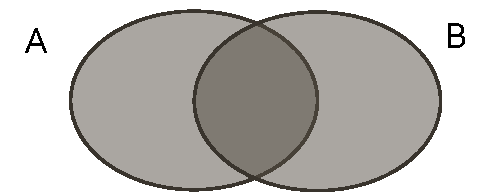
\includegraphics[width=0.25\textwidth]{../assets/img/union.pdf}
            \caption*{L’union de l’ensemble A et B}
            \label{Fig:union}
        \end{center}
    \end{figure}
\end{frame}

\begin{frame}{\secname : \subsecname}
    Exemple
    \begin{itemize}
        \item $A = \{2,3,4,5 \}$
        \item $B = \{1,3,6,8 \}$
        \item $C = \{2,5,10 \}$
    \end{itemize}
    \begin{equation}\footnote{Attention, pas de doublons dans les ensembles, contrairement à Oracle.}
        \begin{split}
            A \cup B & = \{ 1, 2, 3, 4, 5, 6, 8\} \\
            B \cup C & = \{2, 3, 4, 5, 10\}
        \end{split}
    \end{equation}
\end{frame}

\subsection{Différence}
\begin{frame}{\secname : \subsecname}
    $$
        X = R_1 - R_2
    $$
    La différence de deux relations $R_1$ et $R_2$ union-compatibles (dans l’ordre $R_1 - R_2$ ) est une relation $X$ contenant les tuples appartenant à $R_1$ et n’appartenant pas à $R_2$.
    $$
        A \setminus B = \{ x | x \in A \land x \notin B \}
    $$
    \begin{figure}
        \begin{center}
            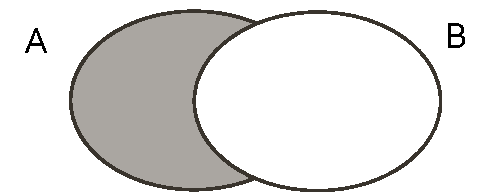
\includegraphics[width=0.25\textwidth]{../assets/img/difference.pdf}
            \caption*{La différence de l’ensemble A et B}
            \label{Fig:difference}
        \end{center}
    \end{figure}
\end{frame}


\begin{frame}{\secname : \subsecname}
    Exemple
    \begin{itemize}
        \item $A = \{2,3,4,5 \}$
        \item $B = \{1,3,6,8 \}$
        \item $C = \{2,5,10 \}$
    \end{itemize}
    \begin{equation}\footnote{$B\setminus C = B$ puisqu'aucune donnée commune entre B et C.}
        \begin{split}
            A \setminus B & = \{ 2, 4, 5 \} \\
            A \setminus C & = \{ 1, 3, 6, 8 \}
        \end{split}
    \end{equation}
\end{frame}


\subsection{Intersection}
\begin{frame}{\secname : \subsecname}
    $$
        X = R_1 \cap R_2
    $$
    L’intersection pouvant s’exprimer en fonction de la différence, cet opérateur n’est pas indispensable\footnote{Nous reviendrons sur l’intersection de deux relations dans le paragraphe des opérateurs additionnels.}.
\end{frame}


\subsection{Produit cartésien}
\begin{frame}{\secname : \subsecname}
    $$
        X = R_1 \times R_2
    $$
    Le produit cartésien de deux relations $R_1$ et $R_2$ (de schéma quelconque) est une relation ayant pour attributs tous les attributs de $R_1$ et de $R_2$ et dont les tuples sont constitués de toutes les concaténations possibles d’un tuple de $R_1$ à un tuple de $R_2$.
    $$
        A \times B = \{(x,y) | x \in A \land y \in B \}
    $$\footnote{Attention, si une relation compte $0$ tuple et l'autre $x$ tuples, le produit cartésien comportera $0$ tuple !}
\end{frame}

\begin{frame}{\secname : \subsecname}
    Exemple
    \begin{itemize}
        \item $A = \{2,3\}$
        \item $B = \{1,3,6 \}$
    \end{itemize}
    \begin{equation}
        \begin{split}
            A \times B & = \{ (2, 1), (2, 3), (2, 6), (3, 1), (3, 3), (3, 6)\} \\
        \end{split}\footnote{Attention, toujours pas de doublons dans les ensembles, contrairement à Oracle.}
    \end{equation}
\end{frame}

\section{Les opérateurs relationnels}
\subsection{Définition}
\begin{frame}{\secname : \subsecname}
    Les deux opérateurs unaires sélection et projection combinés avec les opérations ensemblistes union, différence et produit cartésien étudiés au paragraphe précédent permettent de définir toutes les expressions correctes de l’algèbre relationnelle.
\end{frame}
\subsection{La projection}
\begin{frame}{\secname : \subsecname}
    $$
        X = Projection(R / C_1,C_2,...,C_p)
    $$
    La projection d’une relation $R$ de schéma $R (C_1, C_2, …, C_n)$ sur les attributs $C_{i1}, C_{i2},..., C_{ip}$ (avec $i,j <> i,k$ et $p < n$) est une relation $R’$ de schéma $R’ (C_{i1}, C_{i2},..., C_{ip})$ dont les tuples sont obtenus par élimination des valeurs des attributs de $R$ n’appartenant pas à $R’$ et par suppression des tuples en double.

    L’opérateur de projection permet donc d’extraire certains attributs d’une relation.  On parle de sélection verticale.
\end{frame}

\begin{frame}{\secname : \subsecname}
    \begin{figure}
        \begin{center}
            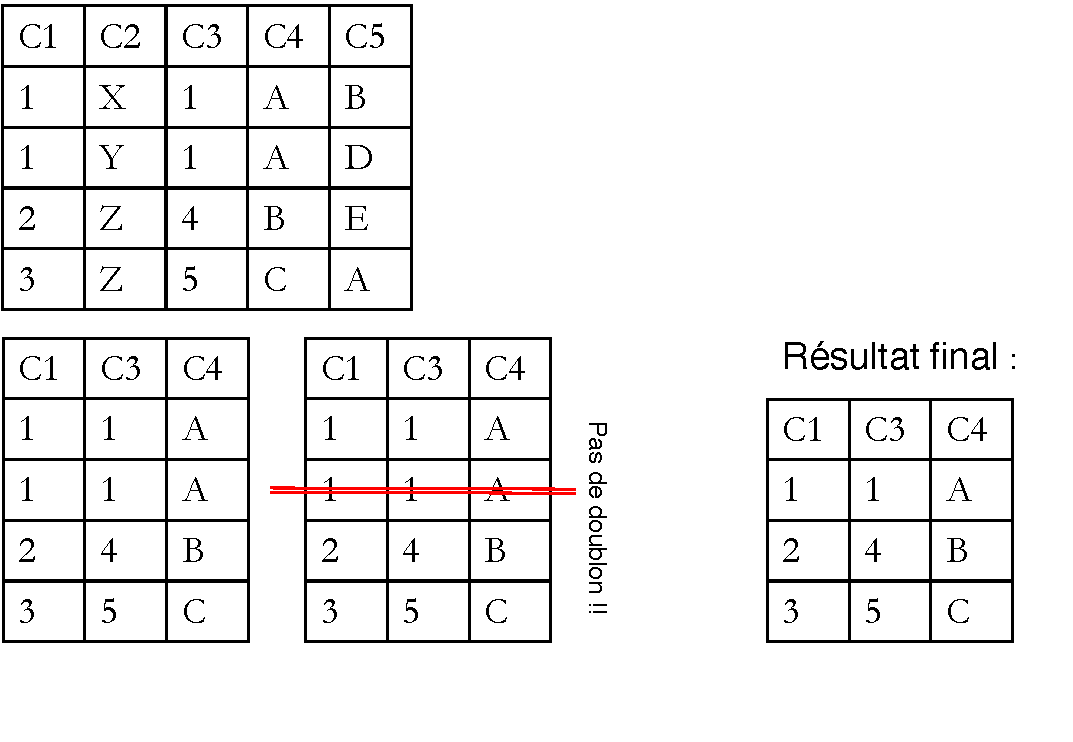
\includegraphics[width=0.65\textwidth]{../assets/img/projection_1.pdf}
            \caption*{Exemple : PROJECTION (R/C1,C3,C4)}
            \label{Fig:projection_1}
        \end{center}
    \end{figure}
\end{frame}

\subsection{La sélection}
\begin{frame}{\secname : \subsecname}
    $$
        X = SELECTION(R / pr\acute{e}dicat)
    $$
    L’opération de sélection, selon un critère $C$, appliquée à une relation $R$ donne une relation $R’$ de même schéma dont les tuples sont ceux de $R$ satisfaisant le critère $C$.

    Critère de sélection : prédicat ou expression logique de prédicats. Chaque prédicat exprime une comparaison entre une colonne d’une table et une constante au moyen d’un opérateur de comparaison.
    \begin{equation}
        \begin{split}
            SELECTION & (livre / Annee = 2010 \land \\
            & NumOuvrage > 3 ET Annee \geq 2005 \land \\
            & (NumOuvrage < 2 ET Annee = 2006) \lor Annee = 2002) \\
        \end{split}
    \end{equation}
\end{frame}

\begin{frame}{\secname : \subsecname}
    \begin{figure}
        \begin{center}
            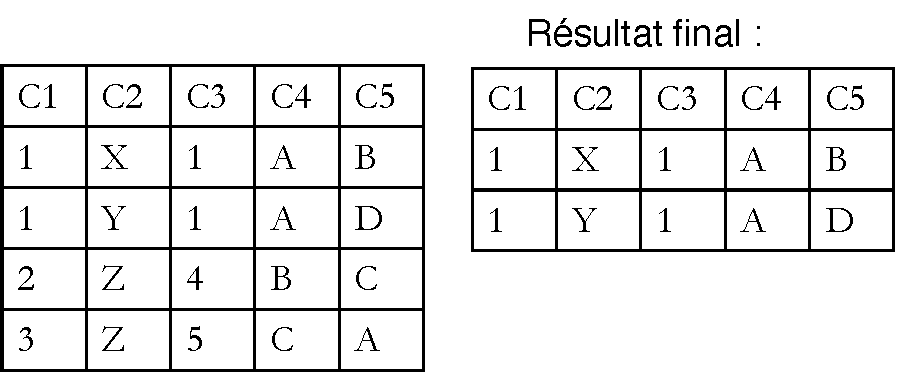
\includegraphics[width=0.5\textwidth]{../assets/img/selection.pdf}
            \caption*{Exemple : SELECTION (R/C4=A)}
            \label{Fig:selection}
        \end{center}
    \end{figure}
\end{frame}

\section{Les opérateurs additionnels}
\subsection{Définition}
\begin{frame}{\secname : \subsecname}
    Les cinq opérateurs vus jusqu'à présent sont suffisants pour exprimer une requête quelconque de l’algèbre relationnelle.  Cependant, certaines requêtes, même banales, sont très longues à exprimer.
    \begin{itemize}
        \item Intersection
        \item Jointure
        \item Jointure externe
        \item Division
    \end{itemize}
\end{frame}

\subsection{Intersection}
\begin{frame}{\secname : \subsecname}
    $$
        X = R_1 \cap R_2
    $$
    L’intersection de deux relations $R_1$ et $R2$ union-compatibles est une relation $X$ contenant les tuples appartenant à $R_1$ et à $R2$.
    $$
        A \cap B = \{ x | x \in A \land x \in B \}
    $$
    \begin{figure}
        \begin{center}
            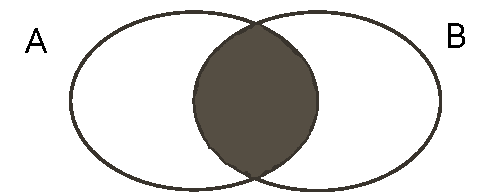
\includegraphics[width=0.35\textwidth]{../assets/img/intersection.pdf}
            \caption{L’intersection}
            \label{Fig:intersection}
        \end{center}
    \end{figure}
\end{frame}

\begin{frame}{\secname : \subsecname}
    $$
        X = R_1 \cap R_2
    $$
    On peut aussi définir l’intersection au moyen de la différence :
    $$
        x = R_1 \setminus (R_1 \setminus R_2) = R_2 \ (R_2 \setminus R_1)
    $$
    \begin{figure}
        \begin{center}
            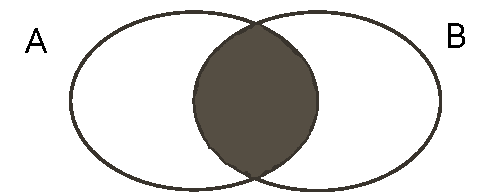
\includegraphics[width=0.35\textwidth]{../assets/img/intersection.pdf}
            \caption{L’intersection}
        \end{center}
    \end{figure}
\end{frame}

\begin{frame}{\secname : \subsecname}
    Exemple
    \begin{itemize}
        \item $A = \{2,3,4,5 \}$
        \item $B = \{1,3,6,8 \}$
        \item $C = \{2,5,10 \}$
    \end{itemize}
    \begin{equation}
        \begin{split}
            A \cap B & = \{3 \} \\
            A \cap C & =  \varnothing
        \end{split}
    \end{equation}
\end{frame}

\begin{frame}{\secname : \subsecname}
    Exemple
    \begin{itemize}
        \item $A = \{2,3,4,5 \}$
        \item $B = \{1,3,6,8 \}$
        \item $C = \{2,5,10 \}$
    \end{itemize}
    \begin{equation}
        \begin{split}
            A \cap B & = A - (A-B) = B- (B-A) \\
            A - B & = \{2, 4, 5\}      A - (A - B) = \{3\} \\
            B - A & = \{1, 6, 8\}      B - (B - A) = \{3\}
        \end{split}
    \end{equation}
\end{frame}


\subsection{Jointure}
\begin{frame}{\secname : \subsecname}
    $$
        X = jointure(R_1,R_2 / C)
    $$
    La jointure de deux relations $R_1$ et $R2$ selon un critère généralisé $C$ est l’ensemble des tuples du produit cartésien $R_1 X R2$ satisfaisant le critère $C$.

    Le critère $C$ est une expression logique de prédicats dans laquelle chaque prédicat exprime une comparaison entre un attribut et une constante ou un attribut et un autre attribut.
    Les attributs comparés doivent impérativement être définis sur des domaines compatibles!
\end{frame}

\begin{frame}{\secname : \subsecname}
    $$
        X = jointure(R_1,R_2 / C)
    $$
    \begin{equation}
        \begin{split}
            x = jointure &(AUTEURS, A\_ECRIT  / \\
            & AUTEURS.NumAuteur = A\_ECRIT.NumAuteur)
        \end{split}
    \end{equation}
    \footnote{Quelles sont les colonnes de l'ensemble $X$ ? Toutes les colonnes de $Auteurs$ et $A\_Ecrit$, sans répétition de la colonne $NumAuteurs$}
\end{frame}

\begin{frame}{\secname : \subsecname}
    Plusieurs cas particuliers de jointures :
    \begin{itemize}
        \item L’équi-jointure de $R_1$ et R2 sur les attributs $C_{R1}$ et $C_{R2}$ est la jointure selon le critère $C_{R1} = C_{R2} ([INNER] JOIN)$\footnote{Le mot-clé INNER JOIN sélectionne les enregistrements qui ont des valeurs correspondantes dans les deux tables.}
        \item L’ auto-jointure de $R$ selon $C_i$ est la jointure de $R$ avec elle-même selon le critère $C = C$
        \item La jointure naturelle de $R_1$ et R2 est l’équijointure de $R_1$ et $R_2$ sur tous les attributs ayant le même nom dans $R_1$ et $R_2$, suivie d’une projection qui permet de conserver un seul de ces attributs égaux de même nom. (NATURAL JOIN)
    \end{itemize}

\end{frame}

\subsection{Jointure}
\begin{frame}{\secname : \subsecname}
    $$
        X = JOIN EXT(R_1,R_2 / C)
    $$
    La jointure externe de deux relations R1 et R2 est obtenue en deux étapes :

    \begin{enumerate}
        \item On effectue une jointure de R1 et R2
        \item On ajoute à la relation obtenue en (1) les tuples de R1 et R2 qui ne participent pas à la jointure complétés avec des valeurs nulles pour les attributs de l’autre relation
    \end{enumerate}
    $$
        ( \{ LEFT | RIGHT | FULL \} OUTER JOIN )
    $$
\end{frame}

\begin{frame}{\secname : \subsecname}
    $$
        X = JOIN EXT(R_1,R_2 / C)
    $$
    \begin{equation}
        \begin{split}
            x = JOIN EXT LEFT &(AUTEURS, A\_ECRIT  / \\
            & AUTEURS.NumAuteur = A\_ECRIT.NumAuteur)
        \end{split}
    \end{equation}
    \footnote{Liste de tous les auteurs et pour ceux qui ont écrit un ou plusieurs ouvrages, un enregistrement pour chaque ouvrage avec l'identifiant de celui-ci en plus des informations concernant l'auteur.}
\end{frame}
\subsection{Division}
\begin{frame}{\secname : \subsecname}
    $$
        X = R_1 \div R_2
    $$
    Le quotient de la relation $R_1$ de schéma $R_1 (C_1, C_2, …, C_p, C_{p+1}, …, C_n)$ par la sous-relation $R_2$ de schéma $R_2 (C_{p+1}, … , C_n)$ est la relation $D$ de schéma $D (C_1, C_2, … C_p)$ formée de tous les tuples qui concaténés à chacun des tuples de $R_2$ donne toujours un tuple de $R_1$.

\end{frame}
\subsection{Exercice}
\begin{frame}{\secname : \subsecname}
    \begin{equation}
        \begin{split}
            PROJECTION_2 &( \\
            JOIN_1 &(Dept, Emp \\
            & / Dept.NrDept = Emp.NrDept) \\
            & / Emp.nom, Dept.nom  )
        \end{split}
    \end{equation}
    \begin{itemize}
        \item Donner le résultat de cette expression.
        \item Quelle est la question à poser pour obtenir ce résultat ?
    \end{itemize}

\end{frame}

\end{document}
